\documentclass[11pt, oneside]{article}   	% use "amsart" instead of "article" for AMSLaTeX format
\usepackage{geometry}                		% See geometry.pdf to learn the layout options. There are lots.
\geometry{letterpaper}                   		% ... or a4paper or a5paper or ... 
%\geometry{landscape}                		% Activate for rotated page geometry
%\usepackage[parfill]{parskip}    		% Activate to begin paragraphs with an empty line rather than an indent
\usepackage{graphicx}				% Use pdf, png, jpg, or eps with pdflatex; use eps in DVI mode
								% TeX will automatically convert eps --> pdf in pdflatex		
\usepackage{amsmath}
\usepackage{mathtools}
\usepackage{amssymb}        % so we can use the 'pretty' empty set
\usepackage{tipa}
\usepackage{graphicx}           % purdy pitchers
\graphicspath{{diagrams/}}
\usepackage{algorithmic}
\usepackage{phonrule}

\usepackage{cite}
\usepackage{apacite}
\usepackage[section]{placeins}

% Reduce in-text citations to 'et al' when there are more than 2 authors
\makeatletter
\usepackage{regexpatch}
\xpatchcmd{\@@cite}{\def\BCA##1##2{{\@BAstyle ##1}}}{\def\BCA##1##2{{\@BAstyle ##2}}}{}{}
\makeatother

\newtheorem{definition}{Definition}

\title{A method for projecting features from observed sets of phonological classes}
\author{}
\author{
  Connor Mayer \\
  \texttt{connormayer@ucla.edu}
  \and
  Robert Daland \\
  \texttt{r.daland@gmail.com}
}
\date{\vspace{-5ex}}							% Activate to display a given date or no date

\begin{document}
\maketitle

\begin{abstract}
This paper describes a collection of dynamic programming algorithms which assign features to a set of phonological classes. The input consists of a set of classes, each containing one or more segments. If a class can be generated as the union of existing features (i.e. as the intersection of already-processed classes), those features are propagated to every segment in the class. A new feature must be assigned otherwise, and we show that this occurs just in case the class has a single parent in the intersectional closure of the input. The algorithm comes in four flavors, which differ with respect to complementation and how negative values are assigned. We show that these variants yield \textit{privative specification}, \textit{contrastive underspecification}, \textit{contrastive specification}, and \textit{full specification}, respectively. This algorithm sheds light on how a feature system may be derived from a set of learned classes, bearing on theories of emergence in phonology and providing testable predictions on the kinds of featurization available to language learners.
\end{abstract}

% LIST OF FIGURES
%	Fig. 1 (done) -- A manner hierarchy class system
%	Fig. 2 (done) -- A vowel inventory
%	Fig. 3 (done) -- Intersectional closure of a vowel inventory
%	Fig. 4 (done) -- Yield of the privative specification algorithm (to Fig. 3)
%	Fig. 5 (done) -- Class system and featurization yielded by contrastive specification
%	Fig. 6 TODO -- Big alphabet (contrastive underspecification with privative, binary, and ternary features)

\section{Introduction}

Features are the substantive building blocks of phonological theory. They represent phonetic qualities of speech sounds, and can be used in isolation or combination to describe individual sounds or classes of sounds \cite<e.g.>{JakobsonEtAl1952, ChomskyHalle1968, Clements1985}.

The goals of feature theory are to capture the following generalizations. First, segments that have common phonetic properties tend to behave alike, both within and across languages. Features allow such commonalities between sounds to be explicitly represented. For example, the English voiceless non-continuants \{p, t, \textipa{\t{tS}}, k\} are all produced with a complete closure of the oral cavity and no vocal fold vibration, and exactly these segments undergo the process of foot-initial aspiration. The feature notation \phonfeat{-continuant \\ -voiced} exposes these shared phonetic properties to the phonological grammar, and the processes which might reference them. More generally, the set of obstruents, which may be specified with the feature \phonfeat{-sonorant}, tends to undergo similar voicing processes across languages (regressive voicing assimilation within obstruent clusters, word-final devoicing, intervocalic and/or postnasal voicing, and so on).

Second, sound changes tend to preserve phonetic qualities of affected sounds, even when the host segment is altered or destroyed. The sub-segmental representation afforded by features allows these changes to be modeled in a principled way. An instance of feature preservation was the fall of the yers in Old Church Slavonic. The front yer (a short, unstressed, high front vowel) deleted in most prosodic positions. However, the preceding consonant typically became palatalized, thereby preserving the high and front articulations, even while the vowel segment was deleted \cite{Carlton1991}. 

Finally, feature theory reflects featural economy and the factorial arrangement of the segmental inventory: if a language treats a particular featural contrast as distinctive, it is likely to be exploited widely throughout its inventory. In other words, segment inventories are more symmetric than might be expected if segments were the atoms of representation \cite<e.g.>{Clements2003}.

Classic texts \cite<e.g.>{ChomskyHalle1968} have assumed phonological features are \textit{universal}: all the sounds in the world's languages can be described by the same finite set of features, which reflect properties of the human vocal tract and perceptual system. According to this view, speakers inherently produce and perceive speech in terms of these features because they are the substantive `atoms' of which segments and higher prosodic constituents are composed. Children represent speech in terms of these atoms, which is why phonological processes operate on the classes they define. Feature theory is manifestly successful in explaining why many common phonological processes involve segments that share relevant phonetic properties.

% ROBERT: Make sure the next few paragraphs don't plagiarize Connor's master's thesis!
However, there is evidence that many phonological processes target sets of segments that cannot be singled out by a set of phonetic properties. A canonical example is the \textit{ruki} rule of Sanskrit, in which an underlying /s/ becomes retroflexed when it occurs later in a word than any of \{r, u, k, i\} \cite<e.g.>{Kiparsky1973, Vennemann1974}. While it has been proposed that the \textit{ruki} process originated from the acoustic effects of these segments on neighboring sounds, e.g. a lowering of the noise frequency of a following /s/ \cite{Longerich1998}, no conventional feature system can pick out all four of these segments to the exclusion of others. The existence of a single, idiosyncratic rule like this is not grounds for theoretical concern. However, it has been proposed that \textit{phonetically disparate classes} like \{r, u, k, i\} are much more common than would be expected under a universal feature system. \citeA{Mielke2008} conducted a survey of phonological processes in almost 600 languages. Of the classes which underwent or conditioned a phonological process, 71\% could be expressed as a combination of simple features by the `best' feature system he considered. To express the remaining 29\%, additional theoretical mechanisms --  such as building classes through an \textsc{OR} operation -- would be needed. These seriously compromise the explanatory power that made feature theory appealing in the first place. 

The purported ubiquity of phonetically disparate classes has led some researchers to propose that distinctive features are \textit{learned} and \textit{language-specific} \cite<e.g.>{Blevins2004, Mielke2008, MacWhinneyOGrady2015, ArchangeliPulleyblank2015}: learners are able to group sounds in their languages into classes, even if they have no phonetic commonality. Under this emergent view of features, the striking regularities that exist across languages are explained as by-products of general human cognitive capabilities, such as categorization, sensitivity to frequency, and the ability to generalize, as well as the properties of the human vocal tract and auditory system.

It is still unclear whether the problematic classes identified by Mielke and others can be captured by other means. It is possible that classes which superficially appear to be phonetically disparate result from interactions between phonological processes that target phonetically coherent classes. Alternatively, these classes may share phonetic similarities that have not yet been formalized in any feature system. Even if these issues are put aside, well established problems like the variable patterning of /l/ as \phonfeat{$+$continuant} or \phonfeat{$-$continuant} across languages suggest that features may be learned to some degree \cite<e.g.>{Kaisse2002, Mielke2008}.

The goal of this paper is not to take a strong position on the correctness of emergent feature theory, but rather to address the question of what a phonological learning system would need to look like under this theory. In constructing such a system, one could start with the features and derive classes, or start with the classes and derive features. Here we develop the latter approach. That is, we suppose that some mechanism has identified particular sets of segments as `candidate' classes -- which we refer to as the input. Several considerations motivate this approach: first, it is unclear how emergent features could be learned without being somehow motivated by the classes they characterize. Second, and more practically, the output of past attempts at unsupervised learning of phonological categories are phonological \textit{classes} \cite<e.g.>{GoldsmithXanthos2009, Calderone2009, Mayer2018}. In principle, a system that learns features from classes allows for the construction of a computational model that takes (minimally) a segmental corpus as input and outputs a featurization of the segmental inventory. This paper describes the final stage of such a model. A related paper, \citeA{Mayer2018}, details an algorithm that takes a phonological corpus and learns classes based on distributional similarity that could serve as the input to this stage.

Below we illustrate how a feature system can be learned from an arbitrary input, i.e. without any reference to the phonetic properties of the segment. We begin in Section \ref{sec:definitions} by formalizing our notation for feature systems. This notation and the lattice-like structures it motivates are similar to past work such as \citeA{Broe1993}, although we provide a more detailed formalism, which aids in proofs of some interesting properties. Section \ref{sec:intersectional} describes the \textit{intersectional closure} of a set of classes, which is necessarily generated by any featurization of that set. Using the intersectional closure as a tool for efficient computation, Sections \ref{sec:privative} to \ref{sec:full} describe a suite of algorithms for learning various types of featurizations for a set of input classes and include proofs of their soundness. Finally, in Section \ref{sec:discussion} we analyze some tradeoffs between the featurization algorithms, and discuss implications for feature theory and feature learning.

This paper makes several contributions. First, it demonstrates a method for working backwards to feature systems underpinning learned classes of sounds. Second, it provides a detailed formalization of feature systems in general. This allows careful reasoning about the expressiveness of such featurizations. Third, by comparing multiple types of algorithms, this work makes explicit predictions about what classes should be describable under each type. Even under a universal theory of features, this will allow future research to precisely investigate the featurizations used by humans. For example, the full specification algorithm predicts that the class of non-nasal sounds should be available to speakers as a byproduct of the nasal class, which suggests that participants in an artificial grammar learning experiment should be able to effectively learn patterns involving this class. The other featurization methods to be discussed do not make this prediction. Finally, it provides the code\footnote{https://github.com/rdaland/Pheatures/} for use and extension in future research. 

\FloatBarrier
\section{Definitions and notation}
\label{sec:definitions}
Let $\Sigma$ denote an alphabet of segments. We will use the term \textit{class} to mean a subset of $\Sigma$.

\subsection{Classes and class systems}

A \textit{class system} $(\mathcal C, \Sigma)$ consists of an alphabet $\Sigma$ and a set of classes $\mathcal C$ over that alphabet. Consider the following simple class system, which is meant to evoke a manner hierarchy.

\vspace{\baselineskip} \noindent \textbf{Example}: Manner hierarchy class system \begin{itemize}
  \item \textit{alphabet} -- \{V, G, L, N, T\}
  \item \textit{sonorants} -- \{V, G, L, N\}
  \item \textit{non-continuants} -- \{N, T\}
  \item \textit{continuants} -- \{V, G, L\}
  \item \textit{singletons} -- \{V\}, \{G\}, \{L\}, \{N\}, \{T\}
  \end{itemize}

\noindent Fig.~\ref{fig:manner_input} illustrates this class system. Each node corresponds to a class. Downward arrows indicate a \textit{parent/child} relationship.

% show an example of a class system: a manner hierarchy
\begin{figure}[h]
  \centering
  \includegraphics[width=0.5\textwidth]{manner_poset_privative.png}
  \caption{A manner hierarchy class system.}
  \label{fig:manner_input}
\end{figure}

\vspace{\baselineskip} \noindent The parent/child relationship is of central importance to this work, so we formalize it carefully here.

\vspace{\baselineskip} \noindent \textbf{Definition}: Let $(\mathcal C, \Sigma)$ be a class system. $X \in \mathcal C$ is a \textit{parent} of $Y \in \mathcal C$ (and $Y$ is a \textit{child} of $X$) if and only if \begin{itemize}
    \item $Y \subset X$, and
    \item there exists no $Z \in \mathcal C$ such that $Y \subset Z \subset X$
    \end{itemize}
In other words, $X$ is a parent of $Y$ if a subset/superset relation holds, and there is no `intervening' class between them. 

In Fig.~\ref{fig:manner_input}, there is a `path' from the alphabet through the sonorants to the continuants. This means the sonorants are a child of the alphabet, and the continuants are a child of the sonorants. The existence of this path implies the continuants are a subset of the alphabet,\footnote{Formally, the subset/superset relation is the \textit{transitive closure} of the parent/child relation, and the parent/child relation is the \textit{transitive reduction} of the subset/superset relation.} but crucially, the continuants are not a child of the alphabet because the sonorants intervene. It is convenient to depict parent/child relationships (rather than subset/superset) to avoid crowding the graph. But this relation is also important for the featurization algorithms we describe later. We additionally define $\textsc{parents}(Y)$ as the set of classes which are parents of a class $Y$, and $\textsc{children}(Y)$ as the set of classes which are children of a class $Y$.

There are some additional aspects of Fig.~\ref{fig:manner_input} which merit comment. First, the empty set is technically a daughter of the singletons (since it is a subset of everything) but it does not appear in the graph. This is because the empty set is a phonologically irrelevant class: it cannot partition the alphabet into segments which undergo a process and those which do not; and to say that it is equivalent to the source or target of a process is equivalent to saying that the process does not happen at all.\footnote{Some confusion may arise with regard to SPE-style rules. In SPE, the null set symbol is used to indicate the source/target of epenthesis/deletion rules. Thus, in SPE the null set symbol is used to denote an \underline{empty string}. In the present work, the null set symbol is used to denote the null set.} Second, the class \{N\} has two dotted arrows which extend to it, rather than a single solid line like the other classes. The dotted lines signify that \{N\} is the intersection of its parents: \{V, G, L, N\} $\cap$ \{N, T\} = \{N\}. As we will prove later, this entails that \{N\} can be expressed as the union of features which express \{V, G, L, N\} and \{N, T\} individually. Therefore, it does not need a new feature to distinguish it from other classes. We will also prove that the converse is true as well: a class needs a new feature just in case it cannot be expressed as the union of the features of its parents. This turns out to mean that a class needs a new feature if and only if it has a single parent. However, this is not guaranteed to be true for the input class system $\mathcal C$; instead, it holds for a derived class system $\mathcal C_\cap$ we call the intersectional closure. Some careful formalization is necessary to express these insights.

\subsection{Feature systems and featurizations}

\textbf{Definition}: A \textit{feature system} is a tuple $(\mathcal F, \Sigma, \mathcal V)$ where \begin{itemize}
    \item $\Sigma$ is a segmental alphabet, 
    \item $\mathcal V$ is a set of values, and 
    \item $\mathcal F$ is a \textit{featurization}: a set of features $\{f_j\}_{j=1}^M$, where each feature is a function $f: \Sigma \rightarrow \mathcal V$ mapping segments to feature values.
    \end{itemize}

\noindent To illustrate, a possible feature system for the manner system of Fig.~\ref{fig:manner_input} is shown below in Table~\ref{table:featurization}. In the next subsection we formalize featural descriptors, which relate classes and feature systems.

\begin{table}[h]
    \centering
    \begin{tabular} {|c||c|c|c|c|}
    \hline
        $\sigma$ & syl & voc & apprx & son \\ \hline
        V & + & + & + & + \\
        G & -- & + & + & + \\
        L & -- & -- & + & + \\
        N & -- & -- & -- & + \\
        T & -- & -- & -- & -- \\
        \hline
    \end{tabular}
    \caption{Example of a feature system.}
    \label{table:featurization}
\end{table}

\subsection{Featural descriptors}

Let $(\mathcal F, \Sigma, \mathcal V)$ be a feature system. We restrict $\mathcal V$ to the following possibilities: \begin{itemize}
    \item \textit{privative specification}: $\mathcal V = \{ +, 0 \}$
    \item \textit{full specification}: $\mathcal V = \{ +, - \}$
    \item \textit{contrastive specification}: $\mathcal V = \{ +, -, 0 \}$
    \end{itemize}

\noindent We will use the notation $\mathcal V_0$ for the set $\mathcal V \setminus \{0\}$, i.e. the set of non-zero values. This is because zero values are a formal mechanism to achieve underspecification, and the theoretical driver for underspecification is the idea that underspecified features are phonologically inactive (i.e. cannot define classes). Then, a \textit{featural descriptor} $\mathbf{e}$ is a set of feature/value pairs where the values cannot be $0$: i.e. $\mathbf{e} \subset \mathcal V_0 \times \mathcal F$. For example, $\mathbf{e} =$  \phonfeat{+front \\ --low} is a featural descriptor. This is an \textit{intensional} description of a class; that is, a description of a class in terms of its properties. The \textit{extension} of a featural descriptor is the set of segments which match (at least) the feature/value pairs in the descriptor. We use angle brackets to indicate this:

$$ \big \langle \mathbf{e} \big \rangle = \{x \in \Sigma \, \mid \, \forall (\alpha_k, f_k) \in \mathbf{e} \text{,  } [ f_k(x) = \alpha_k ] \} $$

\vspace{\baselineskip} \noindent Note that under this definition, the extension of the empty featural descriptor is $\Sigma$, since the predicate is vacuously true for all segments when $\mathbf{e}$ is empty. 

We use the notation $\mathcal V_0^\mathcal F$ to denote the powerset of $\mathcal V_0 \times \mathcal F$, i.e. the set of all licit featural descriptors. Lastly, we define $\langle \mathcal V_0^\mathcal F \rangle = \{ \langle \mathbf{e} \rangle \, \mid \, \mathbf{e} \in \mathcal V_0^\mathcal F \}$, the set of all classes described by some featural descriptor in $\mathcal V_0^\mathcal F$. We say that the feature system $(\mathcal F, \Sigma, \mathcal V)$ generates the class system $\langle \mathcal V_0^\mathcal F \rangle$.

Note that while every featural descriptor in $\mathcal V_0^\mathcal F$ picks out a class in $\langle \mathcal V_0^\mathcal F \rangle$, the two are not generally in 1-1 correspondence. This is because the same class can often be described by multiple featural descriptors. For example, under the the feature system of Table~\ref{table:featurization}, the featural descriptor \phonfeat{+voc} picks out the same class as the featural descriptor \phonfeat{+voc \\ +son}, namely \{V, G\}. Moreover, the featural descriptors \phonfeat{+syl \\ --syl} and \phonfeat{+syl \\ --son} both pick out the empty set.

\vspace{\baselineskip} We say that a feature system $(\mathcal F, \Sigma, \mathcal V)$ \textit{covers} a class system $(\mathcal C, \Sigma)$ if $\mathcal C \subset \langle \mathcal V_0^\mathcal F \rangle$; in other words if the feature system provides a distinct featural representation for every class in $\mathcal C$. In the next subsection, we work an example to illustrate the importance of the choice of the value set in featurization.

\subsection{Example: Sonorants and obstruent voicing}

In this subsection we introduce a simple, 3-segment class system to illustrate the notation, as well as the difference between the privative and full specification value sets.

Let $\Sigma =$ \{R, D, T\}, where $R$ is meant to evoke a sonorant, $D$ a voiced obstruent, and $T$ a voiceless obstruent. Accordingly we use the feature names $vcd$ and $son$, but note that these descriptive labels are purely for the reader's convenience. We begin with the featurization using the private value set, shown in Table~\ref{table:privative}.

% table with featurization of sonorants, voiced obstruents, and voiceless obstruents
\begin{table}[h]
    \centering
    \begin{tabular} {|c||c|c|}
    \hline
        $\sigma$ & son & vcd \\ \hline
        R & + & + \\
        D & 0 & + \\
        T & 0 & 0 \\
        \hline
    \end{tabular}
    \caption{Sonorants and obstruents with privative specification.}
    \label{table:privative}
\end{table}

\noindent The set of classes it describes, and the simplest featural descriptor for each, are shown below: \begin{itemize}
  \item $\langle \, [\,] \, \rangle = $ \{R, D, T\}
  \item $\langle \, [+\text{son}] \, \rangle$ = \{R\}
  \item $\langle \, [+\text{vcd}] \, \rangle$ = \{R, D\}
  \end{itemize}
  
\noindent Note that this featurization provides (i) no featural descriptor that uniquely picks out the voiceless obstruent \{T\}, (ii) no way to pick out the obstruents \{T\} and \{D\} to the exclusion of \{R\}, (iii) no way to pick out the voiced obstruent \{D\} without \{R\}, and (iv) no way to pick out the empty set.

Next, consider the featurization in which the `$0$'s from Table~\ref{table:privative} are replaced with `$-$'s (the full specification value set):

% table with featurization of sonorants, voiced obstruents, and voiceless obstruents
\begin{table}[h]
    \centering
    \begin{tabular} {|c||c|c|}
    \hline
        $\sigma$ & son & vcd \\ \hline
        R & + & + \\
        D & -- & + \\
        T & -- & -- \\
        \hline
    \end{tabular}
    \caption{Sonorants and obstruents with full specification.}
    \label{table:full}
\end{table}

\noindent This featurization is more expressive than the last one: \begin{itemize}
    \item $\langle \, [\,] \, \rangle =$ \{R, D, T\}
    \item $\langle \, [+\text{son}] \, \rangle =$ \{R\}
    \item $\langle \, [-\text{son}] \, \rangle =$ \{D, T\}
    \item $\langle \, [+\text{vcd}] \, \rangle =$ \{R, D\}
    \item $\langle \, [-\text{vcd}]  \, \rangle=$ \{T\}
    \item $\langle \, [-\text{son},+\text{vcd}] \, \rangle =$ \{D\}
    \item $\langle \, [+\text{son},-\text{vcd}] \, \rangle = \varnothing$
    \end{itemize}

\vspace{\baselineskip} \noindent While the privative featurization just covers three classes, the full specification featurization covers six (not counting the empty set). The ability for featural descriptors to refer to `--' values provides a greater number of ways to `slice and dice' the alphabet. It follows that featurizations which assign more `$0$' values generally require more distinct feature functions to cover the same class system.

\vspace{\baselineskip} In the next section, we introduce the notion of intersectional closure. This data structure will prove essential for efficiently assigning feature systems.

\FloatBarrier
\section{Intersectional closure}
\label{sec:intersectional}

In this section we define the \textit{intersectional closure} of a class system $\mathcal{C}$ as the set of classes that can be generated by intersecting $\Sigma$ with an arbitrary subset of classes in $\mathcal{C}$. We relate the intersectional closure to features by showing that if a feature system is expressive enough to generate all the classes in $\mathcal{C}$, it generates the intersectional closure. Then we give a dynamic programming algorithm which efficiently computes the intersectional closure. 

\subsection{Definitions}

\textbf{Definition}: A collection of sets $\mathcal C$ is \textit{intersectionally closed} if and only if for all $X \in \mathcal C$ and $Y \in \mathcal C$, $X \cap Y \in \mathcal C$.

\vspace{\baselineskip} \noindent The \textit{intersectional closure} of a class system $(\mathcal C, \Sigma)$, written $\mathcal C_\cap$, is the smallest intersectionally closed class system which contains $\mathcal C$ and $\Sigma$.

\vspace{\baselineskip} \noindent \textbf{Definition}: $\mathcal C_\cap = \{ \, \big( \bigcap_{X_i \in P} X_i \big) \, \mid \, P \in \mathcal P(\mathcal C \cup \{ \Sigma \}) \}$ where $\mathcal P(\cdot)$ is the powerset operator. 

\vspace{\baselineskip} \noindent In other words, the intersectional closure contains every class which can be generated by finite intersections of classes from $\mathcal C$ (and $\Sigma$), and no other classes besides these.

To illustrate this concept, we introduce the vowel inventory in Table~\ref{table:vowel_inventory}. This class system will serve as a running example throughout the next four sections.

\begin{table}[h]
    \centering
    \begin{tabular} {|c|c|c|c|}
    \hline
                 &            front                   & mid           & back         \\ \hline
         high & \textipa{i} \textipa{y}      &                  & \textipa{u} \\
         mid  & \textipa{E} \textipa{\oe} &                  & \textipa{o} \\
         low  &                                       & \textipa{a} &                  \\ \hline
    \end{tabular}
    \caption{Vowel inventory}
    \label{table:vowel_inventory}
\end{table}

\vspace{\baselineskip} \noindent Let $(\mathcal C, \Sigma)$ consist of the following classes: \begin{itemize}
  \item \textit{alphabet} -- \{\textipa{i}, \textipa{y}, \textipa{u}, \textipa{E}, \textipa{\oe}, \textipa{o}, \textipa{a}\} 
  \item \textit{non-low} -- \{\textipa{i}, \textipa{y}, \textipa{u}, \textipa{E}, \textipa{\oe}, \textipa{o}\} 
  \item \textit{high} -- \{\textipa{i}, \textipa{y}, \textipa{u}\}
  \item \textit{front} -- \{\textipa{i}, \textipa{y}, \textipa{E}, \textipa{\oe}\}
  \item \textit{round} -- \{\textipa{y}, \textipa{u}, \textipa{\oe}, \textipa{o}\}
  \item \textit{singletons} -- \{\textipa{i}\}, \{\textipa{y}\}, \{\textipa{u}\}, \{\textipa{E}\}, \{\textipa{\oe}\}, \{\textipa{o}\}, \{\textipa{a}\}
  \end{itemize}

\vspace{\baselineskip} \noindent $\mathcal C$ is depicted in Fig.~\ref{fig:vowel_inventory}; the intersectional closure $\mathcal C_\cap$ is depicted in Fig.~\ref{fig:vowel_inventory_closure}. The difference between the two is highlighted by using red circles for the `extra' classes.

\begin{figure}[h]
  \centering
  \includegraphics[width=0.8\textwidth]{vowel_inventory_base.png}
  \caption{A vowel inventory.}
  \label{fig:vowel_inventory}
\end{figure}

\begin{figure}[h]
  \centering
  \includegraphics[width=0.7\textwidth]{vowel_inventory_closure.png}
  \caption{Intersectional closure of the vowel inventory.}
  \label{fig:vowel_inventory_closure}
\end{figure}

The key difference is that the intersectional closure contains several 2-segment classes which are the intersection of larger classes. For example, the \textit{high, front} class \{\textipa{i}, \textipa{y}\} is the intersection of the \textit{high} class and the \textit{front} class:

$$ \text{\{\textipa{i}, \textipa{y}\}} = \text{\{\textipa{i}, \textipa{y}, \textipa{u}\}} \cap \text{\{\textipa{i}, \textipa{y}, \textipa{E}, \textipa{\oe}\}} $$

\vspace{\baselineskip} \noindent Note that the high, front, round class \{\textipa{y}\} has dotted lines because it is the intersection of the high/front, front/round, and high/round classes. In the next subsection, we prove that featurizations must cover intersectional closures, i.e. if a featurization is expressive enough to cover $\mathcal C$, it covers $\mathcal C_\cap$.

\subsection{Feature systems generate an intersectional closure}

There is a dual relationship between featural descriptors and the classes they describe: intersection of classes corresponds to union of featural descriptors. We formalize this property with the following lemma.

\vspace{\baselineskip} \noindent \textbf{Featural Intersection Lemma}

Let $(\mathcal F, \Sigma, \mathcal V)$ be a feature system. If $\mathbf{e}_i, \mathbf{e}_j \in \mathcal V_0^\mathcal F$, then $\langle \mathbf{e}_i \cup \mathbf{e}_j \rangle =  \langle \mathbf{e}_i \rangle \cap \langle \mathbf{e}_j \rangle$.

\vspace{\baselineskip} \noindent \textit{Proof}:

The proof proceeds by showing that $ \langle \mathbf{e}_i \rangle \cap \langle \mathbf{e}_j \rangle \subset \langle \mathbf{e}_i \cup \mathbf{e}_j \rangle$ and $\langle \mathbf{e}_i \cup \mathbf{e}_j \rangle \subset  \langle \mathbf{e}_i \rangle \cap \langle \mathbf{e}_j \rangle$.
Let $C_i = \langle \mathbf{e}_i \rangle$ and $C_j = \langle \mathbf{e}_j \rangle$.
First, suppose $x \in C_i \cap C_j$. Then $x \in C_i$. By definition, $x$ must have the features in $\mathbf{e}_i$.
Similarly, $x \in C_j$, and therefore must have the features in $\mathbf{e}_j$.
Thus, $x$ has the features in $\mathbf{e}_i \cup \mathbf{e}_j$. This shows that $C_i \cap C_j \subset \langle \mathbf{e}_i \cup \mathbf{e}_j \rangle$.
Now, suppose $x \in \langle \mathbf{e}_i \cup \mathbf{e}_j \rangle$. Then $x$ has all the features of $\mathbf{e}_i$, and so $x \in C_i$.
Similarly, $x$ has all the features of $\mathbf{e}_j$, so $x \in C_j$. Therefore $x \in C_i \cap C_j$. This shows that $\langle \mathbf{e}_i \cup \mathbf{e}_j \rangle \subset C_i \cap C_j$.
Since both $C_i \cap C_j$ and $\langle \mathbf{e}_i \cup \mathbf{e}_j \rangle$ are subsets of each other, they are equal.
$\square$

\vspace{\baselineskip} We illustrate this lemma with reference to the vowel inventory system introduced above. For concreteness, let us adopt the following featurization:

% table with featurization of sonorants, voiced obstruents, and voiceless obstruents
\begin{table}[h]
    \centering
    \begin{tabular} {|c||c|c|c|c|}
    \hline
        $\sigma$      & low & front & round & high \\ \hline
        \textipa{i}      & --          & +      & 0        & +      \\
        \textipa{E}    & --          & +      & 0         & --      \\
        \textipa{\oe} & --          & +      & +         & --      \\
        \textipa{y}    & --          & +      & +         & +       \\
        \textipa{u}    & --          & --      & +         & +      \\
        \textipa{o}    & --          & --      & +         & --      \\
        \textipa{a}    & +          & 0      & 0         & 0       \\ \hline
    \end{tabular}
    \caption{A featurization of the vowel inventory. The low vowel is unspecified for front/round/high features; the round feature is privative.}
    \label{table:vowel_inventory_underspec}
\end{table}

\vspace{\baselineskip} \noindent Let $\mathbf{e}_1 =$ \phonfeat{+front} and $\mathbf{e}_2 =$ \phonfeat{+round}. Then we have: \begin{itemize}
    \item $\langle \mathbf{e}_1 \rangle = \langle$\phonfeat{+front}$\rangle =$ \{\textipa{\oe}, \textipa{y}, \textipa{E}, \textipa{i}\}
    \item $\langle \mathbf{e}_2 \rangle = \langle$\phonfeat{+round}$\rangle =$ \{\textipa{\oe}, \textipa{o}, \textipa{y}, \textipa{u}\}
    \end{itemize}
\noindent For these values, the Featural Intersection Lemma cashes out as follows: `the set of vowels that are both front and round' is the intersection of `the set of vowels that are front' and `the set of vowels that are round': \begin{itemize}
    \item $\langle \mathbf{e}_1 \rangle \cap \langle \mathbf{e}_2 \rangle =  \langle$\phonfeat{+front}$\rangle \cap \langle$\phonfeat{+round}$\rangle =$ \{\textipa{\oe}, \textipa{y}, \textipa{E}, \textipa{i}\} $\cap$ \{\textipa{\oe}, \textipa{o}, \textipa{y}, \textipa{u}\} = \{\textipa{\oe}, \textipa{y}\}
    \item $\langle \mathbf{e}_1 \cup \mathbf{e}_2 \rangle = \langle$\phonfeat{+front,+round}$\rangle =$ \{\textipa{\oe}, \textipa{y}\}
    \end{itemize}

\noindent The Featural Intersection Lemma proves that this kind of relationship holds for any pair of featural descriptors and the classes they describe.

An important consequence of this lemma is that it can be applied inductively, to relate the union of multiple featural descriptors with the intersection of multiple classes. Because the intersectional closure is defined as the intersection of arbitrarily many classes in an input $\mathcal C$, the Featural Intersection Lemma ends up entailing that if a featurization covers $\mathcal C$, it must cover the intersectional closure.

\vspace{\baselineskip} \noindent \textbf{Intersectional Closure Covering Theorem}

Let $(\mathcal C, \Sigma)$ be a class system and $(\mathcal F, \Sigma, \mathcal V)$ a feature set. If $\mathcal C \subset \langle \mathcal V_0^\mathcal F \rangle$, then $\mathcal C_\cap \subset\langle \mathcal V_0^\mathcal F \rangle $.

\vspace{\baselineskip} \noindent \textit{Proof}:

Let $Y$ be an arbitrary class in $\mathcal C_\cap$. By definition of $\mathcal C_\cap$, there exist $\{X_i \in \mathcal C\}_{i \in I}$ (for some index set $I$, hereafter omitted) such that $Y = \bigcap_i \, X_i$. The hypothesis that $\mathcal C \subset \langle \mathcal V_0^\mathcal F \rangle $ implies that for every such $X_i$, there exists a featural descriptor $\mathbf{e}_i$ such that $\langle \mathbf{e}_i \rangle = X_i$. Thus, $Y = \bigcap_i X_i = X_1 \cap X_2 \cap \ldots \cap X_n$ can also be written $C = \bigcap_i \, \langle \mathbf{e}_i \rangle = \langle \mathbf{e}_1 \rangle \cap \langle \mathbf{e}_2 \rangle \cap \ldots \cap \langle \mathbf{e}_n \rangle$. It follows by induction using Featural Intersection Lemma that $Y = \langle \bigcup_i \mathbf{e}_i \rangle$:

$Y = \langle \mathbf{e}_1 \rangle \cap  \langle \mathbf{e}_2 \rangle \cap \ldots \cap  \langle \mathbf{e}_n \rangle$

\quad $ = \langle \mathbf{e}_1 \cup \mathbf{e}_2 \rangle \cap \mathbf{e}_3 \cap \ldots \cap \langle \mathbf{e}_n \rangle$

\quad $ = \langle \mathbf{e}_1 \cup \mathbf{e}_2 \cup \mathbf{e}_3 \rangle \cap \ldots \cap \langle \mathbf{e}_n \rangle$

\quad $\ldots$

\quad $= \langle \mathbf{e}_1 \cup \mathbf{e}_2 \cup \ldots \cup \mathbf{e}_n \rangle$

\quad $= \langle \bigcup_i  \mathbf{e}_i \rangle$

\vspace{\baselineskip} \noindent The preceding chain of logic demonstrates the following fact: if a class can be expressed as the intersection of classes in $\mathcal C$, then its features are the union of the features in each of those classes. The intersectional closure is defined as all possible intersections of classes in $\mathcal C$. Thus, if $(\mathcal F, \Sigma, \mathcal V)$ covers $\mathcal C$, it covers the intersectional closure. $\square$

Having illustrated the formal notation for features and the notion of intersectional closure, we turn now to a dynamic programming algorithm for efficiently calculating the intersectional closure.

\subsection{An algorithm for calculating the intersectional closure}

The following algorithm yields the intersectional closure of a class system $(\mathcal C, \Sigma)$. It bears a close resemblance to Dijkstra's shortest-paths algorithm \cite{Dijkstra1959}; a proof of soundness is given in the Appendix.

\noindent \begin{algorithmic}
    \ENSURE $\mathcal C_\cap$ is the intersectional closure of the input $\mathcal C$
    \STATE
    \STATE $\mathcal C_\cap \leftarrow \{ \Sigma \} $
    \STATE $\mathcal Q \leftarrow \mathcal C$
    \STATE
    \WHILE{$\mathcal Q \neq \varnothing$}
        \STATE $X \leftarrow \textsc{dequeue}(\mathcal Q)$
        \IF{\NOT $X \in \mathcal C_\cap$}
            \FOR{$Y \in \mathcal C_\cap$}
                \STATE $\textsc{enqueue}(\mathcal Q, X \cap Y)$
            \ENDFOR
            \STATE $\textsc{append}(\mathcal C_\cap, \, X)$
        \ENDIF
    \ENDWHILE
\end{algorithmic}


\subsection{Parenthood in the intersectional closure}

As we will see shortly, the advantage of explicitly computing the intersectional closure is that \textit{a new feature is required for all and only the classes which have a single parent in the intersectional closure}. The core reason for this is that if a class has two parents, it must be their intersection. We prove this here.

\vspace{\baselineskip} \noindent \textbf{Single Parenthood Theorem}

Let $(\mathcal C, \Sigma)$ be a class system and $Y \in \mathcal C_\cap$. If $X_1, X_2 \in \textsc{parents}(Y)$, then $Y = X_1 \cap X_2$.

\vspace{\baselineskip} \noindent \textit{Proof}:

First, observe that $Y \subset X_1 \cap X_2$. This follows trivially from the definition of parenthood: $X_1$ is a parent of $Y$ implies $Y \subset X_1$, $X_2$ is a parent of $Y$ implies $Y \subset X_2$, and so every element in $Y$ is in both $X_1$ and $X_2$.

Now suppose that $X_1 \cap X_2 \neq Y$. The preceding logic showed that either the two are equal, or $Y$ is a proper subset of $X_1 \cap X_2$. But the latter case creates a contradiction. By definition, $X_1 \cap X_2$ must be in the intersectional closure, and $X_1 \cap X_2 \subset X_1$ follows from fundamental properties of sets. Then $X_1 \cap X_2$ intervenes between $Y$ and $X_1$, contradicting the hypothesis that $Y$ is a daughter of $X_1$. Thus, $Y = X_1 \cap X_2$. $\square$
	
\vspace{\baselineskip} Note that the Single Parenthood Theorem does not logically exclude the possibility that a class may have more than two parents. Rather, it guarantees that in such cases, the intersection is the same regardless of how many parents are considered. One case in which this can happen is the null set: if $x, y, z$ are three distinct elements from $\Sigma$, then $\{ x \} \cap \{ y \} = \varnothing = \{ y \} \cap \{ z \}$. A more interesting case arose already in Fig.~\ref{fig:vowel_inventory_closure}, the intersectional closure of the vowel inventory. There, the three features \textit{front}, \textit{high}, and \textit{round} give rise to three distinct 2-feature classes (featural descriptors: \phonfeat{+front \\ +high}, \phonfeat{+high \\ +round}, \phonfeat{+round \\ +front}). The intersection of any pair of these is \{\textipa{y}\} (the high, front, round vowel). Thus, the set  \{\textipa{y}\} has three parents, but which segments it contains is uniquely determined by any two of them.

With the necessary structures and notation in place, we now turn to the main question addressed in this paper: given a set of phonological classes, how can we generate a covering feature system? We detail four algorithms that accomplish this, differing in their assumptions about a few properties of the featurization. In the next section, we describe the first and simplest of these: an algorithm that generates a privative feature system that covers the intersectional closure $\mathcal C_\cap$, given the input of a class system $(\mathcal C, \Sigma)$.

\FloatBarrier
\section{Privative specification}
\label{sec:privative}

The following algorithm yields a \textit{privative} featurization of a set of classes: that is, one where the set of legal feature values $\mathcal V = \{+, 0\}$. It does so by assigning a different feature/value pair, \phonfeat{$+f$}, to the segments in each class with a single parent.
 
\noindent \begin{algorithmic}
    \REQUIRE $\mathcal C_\cap$ is the intersectional closure of a class system $(\mathcal C, \Sigma)$
    \ENSURE $\mathcal F$ is a featurization over $\mathcal V = \{ +, 0 \}$ which covers $\mathcal C$
    \STATE
    \STATE $\mathcal Q \leftarrow \mathcal C_\cap$
    \STATE $\mathcal F \leftarrow \varnothing$
    \STATE
    \WHILE{$\mathcal Q \neq \varnothing$}
        \STATE $X \leftarrow \textsc{pop}(\mathcal Q)$
        \IF{$|\textsc{parents}(X)| = 1$}
            \STATE define $f_X : \Sigma \rightarrow \mathcal V$ by $f_X(\sigma) = \begin{cases}
                + & \mbox{if } \sigma \in X \\
                0 & \mbox{otherwise}
                \end{cases} $
            \STATE $\textsc{append}(\mathcal F, f_X)$
        \ENDIF
    \ENDWHILE
\end{algorithmic}

\vspace{\baselineskip} \noindent \textit{Proof of soundness for the privative specification algorithm}

A featurization algorithm is \textit{sound} if for every class system $(\mathcal C, \Sigma)$, it returns a feature system which covers $\mathcal C$. To see that the privative specification algorithm is sound, note that every class in $\mathcal C_\cap$ enters the queue $\mathcal Q$. For an arbitrary class $X$ in the queue, there are 3 cases. If $X$ has 0 parents, then it is $\Sigma$, and is covered by the empty featural descriptor. If $X$ has exactly 1 parent, then the segments in $X$ get the features of that parent (which uniquely pick out the parent class), plus a new feature $f$ which distinguishes the segments in $X$ from $X$'s parent. If $X$ has more than 1 parent, then Single Parenthood Theorem shows, via the Featural Intersection Lemma, that the union of features of $X$'s parents uniquely pick out all and only the segments in $X$. Thus, each class which exits the queue has a set of features assigned to its segments which pick out that class uniquely. This completes the proof. $\square$

\vspace{\baselineskip} In Fig.~\ref{fig:privative}, we illustrate the outcome of applying the privative specification algorithm to (the intersectional closure of) the vowel class inventory shown in Fig.~\ref{fig:vowel_inventory_closure}. We employ several conventions to jointly optimize readability and informativity. First, classes which have a single parent are visually highlighted using a thick, red border. These represent the classes that cannot be featurized simply by the union of their parents' features. Second, the arrow which leads to each such class is annotated with the feature/value pair that is used to distinguish it. This represents the `point' at which each feature is assigned. This could give the misleading impression that features are assigned to classes; so it is worth reinforcing here that features are maps from \textit{segments} to values. As a consequence, when the algorithm assigns a feature/value pairs to every segment in a class, the feature/value pair is automatically inherited by every descendant of the class. The set of features that is shared by all members of a class is represented under the node. The complete featurization assigned to each segment is thus represented by inspecting the singleton sets in the bottom row. For readability, we use feature names that are familiar from phonological theory when the feature picks out more than segment in isolation (but note that the algorithm knows nothing of phonetic substance -- as far as it is concerned, they are just arbitrary symbols). When the feature only picks out one segment, we name the feature after the segment.

% ROBERT: This needs to be redone to include the [-low] class. I included the basic feature diagram here as a placeholder/starting point. The .gv file is in the diagrams folder if it's a useful. If you decide to start from your original file instead, make sure you convert it to 300 dpi.
\begin{figure}[htb!]
  \centering
  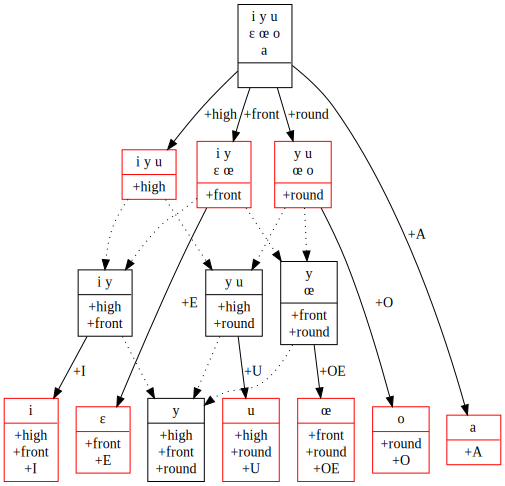
\includegraphics[width=0.9\textwidth]{vowel_inventory_privative.png}
  \caption{Yield of the privative specification algorithm.}
  \label{fig:privative}
\end{figure}

We close this section with some observations on the properties of the privative specification algorithm and the featurization it yields. 

\subsection{Properties of privative specification}
\label{sec:priv_props}

One point to observe is that the privative specification algorithm is \textit{maximally conservative}. What we mean by this is that the resulting feature system generates the smallest class system that covers $\mathcal C$. As the Intersectional Closure Covering Theorem showed, any featurization which covers $\mathcal C$ will cover $\mathcal C_\cap$. This means that any classes which are the intersection of input classes, but which were not themselves in the input, will be `accessible' to the output feature system. But the privative specification algorithm will not make it possible to refer to any other classes outside the intersectional closure. For example, if the input contains a \phonfeat{+front} class and a \phonfeat{+round} class, it must generate a \phonfeat{+front \\ +round} class, but it will not `create' a \phonfeat{--round} class.

This might be the desired behavior. But other properties might be desired instead. For instance, one might have theoretical grounds for wishing to allow `$-$' values. One might also wish to have an \textit{efficient} feature system -- one which minimizes the number of features needed to cover $\mathcal C$. It is easy to show that one can sometimes achieve a more efficient feature system by adding classes to the system. For example, the featurization shown in Fig.~\ref{fig:privative} contains ten features: \textit{low}, \textit{non-low}, \textit{front}, \textit{high}, \textit{round}, plus five features for the individual segments that cannot be accessed as combinations of these features (note that /y/ alone can be uniquely specified using some combination of these). If the input consists of the following classes, the privative specification algorithm returns a featurization with eight features:\footnote{We will not prove this here, but you might enjoy doing this yourself using the descriptions of the intersectional closure and privative algorithm given above.}

 \begin{itemize}
	\item \textit{alphabet} -- \{\textipa{i}, \textipa{y}, \textipa{u}, \textipa{E}, \textipa{\oe}, \textipa{o}, \textipa{a}\} 
	\item \textit{non-low} -- \{\textipa{i}, \textipa{y}, \textipa{u}, \textipa{E}, \textipa{\oe}, \textipa{o}\} 
    \item \textit{front} -- \{\textipa{i}, \textipa{y}, \textipa{E}, \textipa{\oe}\}
    \item \textit{back} -- \{\textipa{u}, \textipa{o}\}
    \item \textit{round} -- \{\textipa{y}, \textipa{u}, \textipa{\oe}, \textipa{o}\}
    \item \textit{unround} -- \{\textipa{i}, \textipa{E}\}
    \item \textit{high} --  \{\textipa{i}, \textipa{y}, \textipa{u}\}
    \item \textit{mid} --  \{\textipa{E}, \textipa{\oe}, \textipa{o}\}
    \item \textit{singletons} -- \{\textipa{i}\}, \{\textipa{y}\}, \{\textipa{u}\}, \{\textipa{E}\}, \{\textipa{\oe}\}, \{\textipa{o}\}, \{\textipa{a}\}
    \end{itemize}
Crucially, this featurization covers the original class system shown in Fig.~\ref{fig:vowel_inventory}. Thus, it uses fewer features while generating a richer class system.

This example is presented to make two points. First, the relationship between classes in the input and the specification algorithm is not monotone. In general, adding features to a system will make more classes accessible -- but in this example, a smaller number of features covers a larger class system. Thus, the minimal number of features needed to cover $\mathcal C$ is not predictable from a `simple' property, such as the total number of classes in $\mathcal C$. To be more precise, the proof of soundness of the privative specification algorithm gives an upper bound on the features needed to cover a class system (namely, the number of classes in the intersectional closure with a single parent). We return to the issue of feature efficiency and expressiveness in Section \ref{sec:discussion}. In the meantime, we turn to the second point this example makes -- adding the `right' classes to the input is what enabled a more economical feature system. In the next sections, we explore variants of the privative specification algorithm which consider complement classes and assign `$-$' values instead of (or in addition to) `$0$' values. 

\FloatBarrier
\section{Contrastive underspecification}
\label{sec:contrastiveunder}

One of the best cases for non-privative specifications arises from complement classes, such as round vs. nonround vowels, or voiced vs. voiceless obstruents. Consider a language with rounding harmony, such as Turkish. Under privative specification one would need to write one harmony rule for the \phonfeat{+round} feature, and an otherwise identical rule for the \phonfeat{+nonround} feature. By allowing features to take on opposing values, one formally recognizes the sameness of rounding with respect to the harmony process.

In canonical cases like rounding harmony and voicing assimilation, the binary feature is only relevant for certain segments. For example, in the case of rounding harmony, it is normally useful to assign the \phonfeat{+round} and \phonfeat{-round} values only to vowels. In some languages, one might wish to only assign these values to just non-low vowels, or just front vowels. In all such cases, the contrasting feature values denote complementary classes -- but complements with respect to \textit{what}?

The central insight developed in this paper is that a new feature needs to be assigned just in case a class has a single parent. This suggests that a relevant domain for complementation is with respect to the parent. This is the distinction between privative specification and contrastive underspecification: a `$-$' value is assigned when the complement of the class being processed with respect to its parent is in the input and has a single parent.

\vspace{\baselineskip} \noindent \begin{algorithmic}
    \REQUIRE $\mathcal C_\cap$ is the intersectional closure of input class system $(\mathcal C, \Sigma)$
    \ENSURE $\mathcal F$ is a featurization over $\mathcal V = \{ +, -, 0 \}$ which covers $\mathcal C$
    \STATE
    \STATE $\mathcal Q \leftarrow \mathcal C_\cap$
    \STATE $\mathcal F \leftarrow \varnothing$
    \STATE
    \WHILE{$\mathcal Q \neq \varnothing$}
        \STATE $X \leftarrow \textsc{dequeue}(\mathcal Q)$
        \IF{$| \textsc{parents}(X) | = 1$}
            \STATE $P_X \leftarrow \textsc{dequeue}(\textsc{parents}(X))$
            \STATE
            \STATE $\overline{X} \leftarrow \begin{cases}
                P_X \setminus X & \text{if } (P_X \setminus X) \in \mathcal C \\
                \varnothing     & \text{otherwise}
                \end{cases}$
            \STATE
            \STATE define $f_X : \Sigma \rightarrow \mathcal V$ by $f_X (\sigma) = \begin{cases}
                    + & \text{if } \sigma \in X \\
                    - & \text{if } \sigma \in \overline{X} \\
                    0 & \text{otherwise}
                    \end{cases}$
            \STATE $\textsc{append}(\mathcal F, f_X)$
            \STATE $\mathcal{Q} \leftarrow \{x \in \mathcal{Q} \vert x \neq \overline{X} \}$
        \ENDIF
    \ENDWHILE
\end{algorithmic}

\vspace{\baselineskip} \noindent The soundness of this algorithm follows from the soundness of the privative specification algorithm. This is because the contrastive underspecification algorithm yields a feature system which generates the same class system as privative specification does. The difference between the two is that if the input contains complement sets, then contrastive underspecification will use a single feature with `$+$' and `$-$' values, where privative specification will have two features with just `$+$' values.

% ROBERT: This is a new figure, and needs to be prettied up similar to the one above.
\begin{figure}[htb!]
	\centering
	\includegraphics[width=0.9\textwidth]{vowel_inventory_contrastive_under.png}
	\caption{Yield of the contrastive underspecification algorithm.}
	\label{fig:vowel_inventory_contrastive_under}
\end{figure}

We illustrate this algorithm using the same vowel system used in the previous section. The featurization using this algorithm is shown in Figure~\ref{fig:vowel_inventory_contrastive_under}. Note that now only nine features are required. The \phonfeat{low} feature, which was privative under the privative specification algorithm, is now binary, because the low and non-low classes are complements with respect to their parent ($\Sigma$), and both are present in the input, and all segments are descendants of one of these classes. Because of this, the \phonfeat{+nonlow} feature from the privative specification is now replaced by \phonfeat{--low}. In addition, some of the features that pick out single segments, \phonfeat{I}, \phonfeat{OE}, and \phonfeat{U}, are now ternary, because /y/ is a complement to the single parent that motivates the addition of these features. Note that the remaining features are still privative because their respective complements are either not present in the alphabet (in the case of \phonfeat{front}, \phonfeat{round}, and \phonfeat{high}).

The term \textit{contrastive underspecification} is meant to capture that features can be binary, ternary, or privative. Segments will be underspecified with respect to a feature if the relevant complement class with respect to a parent is not included in the input. If the additional complement classes described in Section \ref{sec:priv_props} were included in the input for the vowel system, fewer features would be required. In the next section, we consider a variant of the algorithm which adds such complement class, even if it was not present in the input. We call this variant \textit{contrastive specification}.

\FloatBarrier
\section{Contrastive specification}
\label{sec:contrastive}

Contrastive specification is very similar to contrastive underspecification. The key difference is that contrastive specification adds complements (with respect to the parent) to the covering. Every complement gets a `$-$' feature, including those which were not in the input. This can result in adding classes that are not in the intersectional closure of the input. One way to address this is to update the intersectional closure dynamically. However, it is also possible to precompute the result (because the classes that must be added can be defined in terms of subset/superset relations, which do not depend on features); we do this as it is conceptually simpler.

We denote the function that adds complement classes with \textsc{AddComplementsContrastive}. When adding complement classes, the ordering in which classes are processed is crucially important. Breadth-first traversal -- processing all the siblings of a class before its children -- is done to avoid configurations that duplicate a feature. In addition, the order in which siblings are processed during breadth-first traversal has important consequences for the generated class and feature systems. We adopt a procedure whereby the complements of all siblings are added \textit{simultaneously} to the class set if they are not already present. This has the potential to result in less efficient featurizations than adding the complements one-by-one as each class is processed, but it avoids imposing class hierarchies that are not motivated by the input class set. A further motivation for this scheme is that if classes are not processed simultaneously, some order must be chosen, and there is no clear motivation for choosing one over another. A detailed description of \textsc{AddComplementsContrastive} and considerations of other variants can be found in Appendix \ref{app:complements}.

\vspace{\baselineskip} \noindent \begin{algorithmic}
    \REQUIRE $\mathcal C_\cap$ is the intersectional closure of input class system $(\mathcal C, \Sigma)$
    \ENSURE $\mathcal F$ is a featurization over $\mathcal V = \{ +, -, 0 \}$ which covers $\mathcal C$
    \STATE
    \STATE $\mathcal Q \leftarrow \textsc{AddComplementsContrastive}(\mathcal{C_\cap})$
    \STATE $\mathcal F \leftarrow \varnothing$
    \STATE
    \WHILE{$\mathcal Q \neq \varnothing$}
        \STATE $X \leftarrow \textsc{dequeue}(\mathcal Q)$
        \IF{$| \textsc{parents}(X) | = 1$}
            \STATE $P_X \leftarrow \textsc{dequeue}(\textsc{parents}(X))$
            \STATE $\overline{X} \leftarrow P_X \setminus X$
            \STATE define $f_X : \Sigma \rightarrow \mathcal V$ by $f_X (\sigma) = \begin{cases}
                    + & \text{if } \sigma \in X \\
                    - & \text{if } \sigma \in \overline{X} \\
                    0 & \text{otherwise}
                    \end{cases}$
            \STATE $\textsc{append}(\mathcal F, f_X)$
            \STATE $\mathcal{Q} \leftarrow \{x \in \mathcal{Q} \vert x \neq \overline{X} \}$
        \ENDIF
    \ENDWHILE
\end{algorithmic}

\vspace{\baselineskip} \noindent This algorithm is sound because it considers all the classes that the privative specification algorithm does, plus others. Thus, it necessarily covers $\mathcal C$.

Fig.~\ref{fig:contrastive} illustrates the contrastive specification algorithm using the vowel system introduced earlier. Now the complement classes with respect to their parent of the round, high, and front classes have been added, resulting in a more efficient and expressive featurization containing only binary or ternary features.

% ROBERT: This figure is still fine, but should be raised to 300 dpi.
\begin{figure}[htb!]
	\centering
	\includegraphics[width=\textwidth]{vowel_inventory_contrastive.png}
	\caption{Class system and featurization yielded by contrastive specification.}
	\label{fig:contrastive}
\end{figure}

Note that the feature system yielded by contrastive specification is much more expressive than the one yielded by privative specification or contrastive underspecification. However, it is not maximally expressive, since it still contains `$0$' values. When a new feature is added, non-zero values are added only to classes that are descendants of the parent of the class that generates the new feature. In the class system above, /a/ is unspecified for all features except \phonfeat{low}, since it is a descendant only of $\Sigma$.

As another example, suppose that stridents are daughters of coronals, and coronals are daughters of $\Sigma$. Then contrastive specification will create a \phonfeat{--coronal} class (all noncoronals) and a \phonfeat{--strident} class. The latter class will include all coronal nonstridents, but it will not include labials or other noncoronal nonstridents. Thus, while the \textit{coronal} feature assigns a `$+$' or `$-$' value to every segment, the \textit{strident} feature assigns a `$0$' value to noncoronals. If it is desired to eliminate all `$0$' values, one can do complementation with respect to $\Sigma$ rather than the single parent. That is the final variant we discuss -- full specification.

\FloatBarrier
\section{Full specification}
\label{sec:full}

Full specification differs from contrastive specification in that complementation is calculated with respect to the whole alphabet, rather than the parent class. Therefore, it is algorithmically almost the same as contrastive specification. As with contrastive specification, the complement classes are precomputed and added to the intersectional closure in breadth-first search order, and siblings are processed simultaneously. We denote this process as \textsc{AddComplementsFull}: see Appendix \ref{app:complements} for a detailed description.

\vspace{\baselineskip} \noindent \begin{algorithmic}
    \REQUIRE $\mathcal C_\cap$ is the intersectional closure of input class system $(\mathcal C, \Sigma)$
    \ENSURE $\mathcal F$ is a featurization over $\mathcal V = \{ +, - \}$ which covers $\mathcal C$
    \STATE
    \STATE $\mathcal Q \leftarrow \textsc{AddComplementsFull}(\mathcal{C_\cap})$
    \STATE $\mathcal F \leftarrow \varnothing$
    \STATE
    \WHILE{$\mathcal Q \neq \varnothing$}
        \STATE $X \leftarrow \textsc{dequeue}(\mathcal Q)$
        \IF{$| \textsc{parents}(X) | = 1$}
	        \STATE $\overline{X} \leftarrow \Sigma \setminus X$
            \STATE define $f_X : \Sigma \rightarrow \mathcal V$ by $f_X (\sigma) = \begin{cases}
                    + & \text{if } \sigma \in X \\
                    - & \text{otherwise}
                    \end{cases}$
            \STATE $\textsc{append}(\mathcal F, f_X)$
            \STATE $\mathcal{Q} \leftarrow \{x \in \mathcal{Q} \vert x \neq \overline{X} \}$
        \ENDIF
    \ENDWHILE
\end{algorithmic}

\vspace{\baselineskip} \noindent The full specification algorithm is sound for the same reason that the contrastive specification algorithm is -- it considers a superset of classes that the privative specification algorithm does, and thus it covers the input.

This featurization is illustrated by Figure~\ref{fig:vowel_inventory_full}, which uses the same vowel system from previous sections. Note that the number of features is the same as the contrastive featurization, but now /a/ is fully specified for all features, and several new classes have been introduced as a consequence, significantly altering the overall structure of the class system.

% ROBERT: This figure needs to be prettied up, as above.
\begin{figure}[htb!]
	\centering
	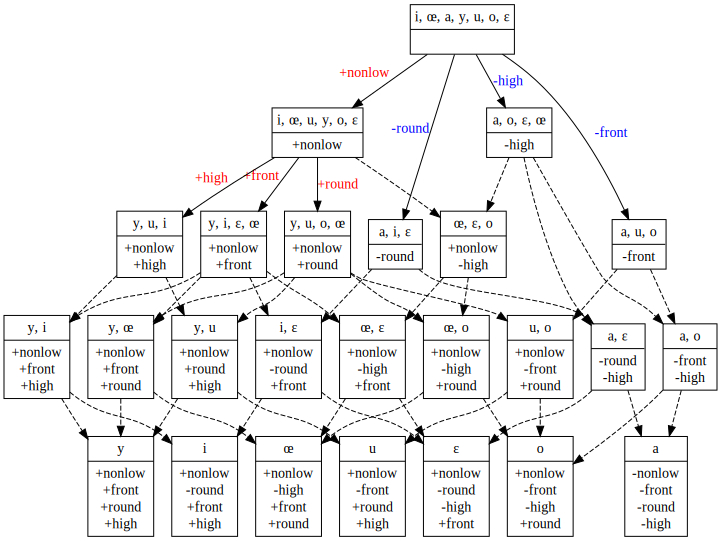
\includegraphics[width=\textwidth]{vowel_inventory_full.png}
	\caption{Class system and featurization yielded by full specification.}
	\label{fig:vowel_inventory_full}
\end{figure}

The key way in which full specification differs from contrastive specification is that no privative specification can occur whatsoever. For example, if a single feature \phonfeat{+nasal} is used to pick out nasal segments, then the feature system will also generate the class \phonfeat{--nasal} consisting of all non-nasal segments. According to our understanding of nasal typology, this is probably not the desired behavior for the nasal feature \cite<e.g.>{Trigo1993}. However, it is possible to avoid generating a \phonfeat{--nasal} class by ensuring that the nasals are generated as the union of pre-existing features, rather than needing their own feature. For example, if \phonfeat{--continuant} picks out the nasals and oral stops, while \phonfeat{+sonorant} picks out vowels, glides, liquids, and nasals, then the nasal class is picked out by \phonfeat{--continuant \\ +sonorant}. Therefore, the set of all non-nasals will not generated as a complement class because the \phonfeat{+nasal} feature is not generated at all. A desirable property of this solution is that the following classes fall out: continuant non-sonorants (fricatives), continuant sonorants (approximants), and non-continuant non-sonorants (stops and affricates). Less desirably, this solution fails to transparently represent nasal spreading processes; for example, vowel nasalization cannot be described as continuancy or sonorancy assimilation. Thus, the cross-linguistic behavior and learnability of classes like \phonfeat{--nasal} has the potential to inform feature theory. We take up this and other issues in Section \ref{sec:discussion}.

\FloatBarrier
\section{Discussion}
\label{sec:discussion}

In this paper, we have described a number of algorithms which assign a featurization to a set of classes, such that every class in the input can be picked out by a featural description. We gave several variants of the algorithm, differing in how conservative they are with respect to the input. The most conservative algorithm assigns a privative specification, i.e. feature functions which only pick out positively specified elements. Contrastive underspecification is achieved with the same algorithm, except that a negative specification is assigned just in case the complement of a class with respect to its parent class is in the input. Contrastive specification is similar, except that a negative specification is assigned even if the complement with respect to the parent was not in the input. Full specification is similar to contrastive specification, except the complement is taken with respect to the entire segmental alphabet. In this section, we discuss some outstanding issues, such as feature economy, how the current work bears on feature theory, and applications toward a richer theory of feature learning.

\subsection{Feature efficiency and expressiveness}

Here we present some examples which illustrate a little more about the expressiveness of class systems.

Let $\mathcal C = \{ \{\sigma\} \, | \, \sigma \in \Sigma \}$; that is, the input consists of all and only the singleton sets. For convenience, we will refer to this as the \textit{singleton input}. Consider what happens when the privative specification algorithm is run on the singleton input. It will yield a featurization with $n$ features, where $n$ is the cardinality of $\Sigma$. This is because each segment gets its own feature, since the only parent of each segment is $\Sigma$. This featurization will generate only the classes in the input (and $\Sigma$, and $\varnothing$).

The opposite extreme is obtained by the \textit{singleton complement} input -- where the input consists not of all singleton sets, but the complement of each singleton set:  $\mathcal C = \{ \Sigma \setminus \{\sigma\} \, | \, \sigma \in \Sigma \}$. It is possible to show that when the privative specification algorithm is given this input, it generates the full powerset of $\Sigma$ -- every possible subset gets a unique combination of features. This follows from the fact that any set can be defined by listing the features for the segments not contained in it. Thus, privative specification is still compatible with a maximally expressive system.

The powerset of $\Sigma$ is also generated by running the full specification algorithm on the singleton input. Thus, there are cases where a more conservative algorithm yields the same class system as a less conservative algorithm (albeit with a different number of features). In fact, it is generally true that the more conservative algorithms can achieve the same level of expressiveness as any less conservative algorithm, by virtue of including the relevant complement classes in the input. For example, if all complement classes with respect to $\Sigma$ are included, the privative specification algorithm yields the same class system as the full specification one does, although with twice the number of features (the singleton complement input discussed above is a special case of this). Moreover, contrastive underspecification, contrastive specification, and full specification all yield the same featurization (as well as the same class system) if every relevant complement class is included. In short, the algorithms can yield radically different class systems depending on their input -- but all can be made highly expressive by tailoring the input appropriately.

\subsection{Relation to feature theory}

As the examples in the preceding section illustrate, the most conservative algorithms (privative specification and contrastive underspecification) are able to yield class systems that are as expressive as the less conservative algorithms. However, the converse is not true. For example, full specification cannot yield a class system as unexpressive as the singleton input does under privative specification. We regard this kind of question as an interesting area for future work, but, as working phonologists, we also want to know: which is the best algorithm to use? Put another way, what matters for feature systems? One principle is that a feature system is good to the extent that learned features render the grammar simpler and/or more insightful. For example, the use of `$+$' and `$-$' values yields insight if both values behave in the same way with respect to a harmony or assimilation process.

The received wisdom of the field generally recognizes the following cases: \begin{itemize}
    \item treat certain features as binary: e.g. all segments are either \phonfeat{+son} or \phonfeat{-son}
    \item treat certain features as privative: e.g. nasals are \phonfeat{+nasal} and all others are \phonfeat{0nasal}
    \item treat most features as ternary: e.g. all obstruents are \phonfeat{+voiced} or \phonfeat{-voiced}, but sonorants are simply \phonfeat{0voiced}
    \end{itemize}
Out of the algorithms we have discussed here, only the contrastive algorithms are capable of yielding a featurization which creates all three feature types. The distinction between contrastive underspecification and contrastive featurizations depends on whether complements of input classes with respect to their parents must also be in the input (which perhaps corresponds to phonological activeness) or can be defined implicitly. This is an issue that can be resolved empirically.

Here are the conditions under which the constrastive underspecification algorithm creates those three types of feature functions:
\begin{itemize}
    \item binary features are generated when a class $X$ and its complement $\Sigma \setminus X$ are both in the input
    \item privative features are generated when a class $X$ is in the input, but no complement (with respect to any ancestor, including its parent, $\Sigma$, and any intervening classes) is
    \item ternary features are generated when a class $X$ is in the input, and its complement $\overline{X}$ with respect to its parent other than $\Sigma$ is in the input
    \end{itemize}

\vspace{\baselineskip} For reasons of space, we do not prove that those are the correct conditions. Instead, we present an example which generates privative, binary, and ternary features. Let $\mathcal C$ include the following: \begin{itemize}
    \item \textit{inventory} -- \{a, i, u, l, r, m, n, \textipa{N}, p, t, k, b, d, g\}
    \item \textit{consonants} -- \{l, r, m, n, \textipa{N}, p, t, k, b, d, g\}
    \item \textit{sonorants} -- \{a, i, u, l, r, m, n, \textipa{N}\}
    \item \textit{obstruents} -- \{p, t, k, b, d, g\}
    \item \textit{coronal} -- \{n, l, r, t, d\}
    \item \textit{vowels} -- \{a, i, u\}
    \item \textit{nasals} -- \{m, n, \textipa{N}\}
    \item \textit{voiceless} -- \{p, t, k\}
    \item \textit{voiced} -- \{b, d, g\}
    \item \textit{labial} -- \{m, p, b\}
    \item \textit{dorsal} -- \{\textipa{N}, k, g\}
    \item \textit{liquids} -- \{l, r\}
    \item \textit{lateral} -- \{l\}
    \item \textit{rhotic} -- \{r\}
    \end{itemize}
The class system that results from running the contrastive underspecification algorithm on this input is shown in Fig.~\ref{fig:big_alphabet}. The features \phonfeat{cons} and \phonfeat{son} are binary because each one partitions $\Sigma$. The features \phonfeat{LAB}, \phonfeat{COR}, \phonfeat{DOR}, \phonfeat{nas} and \phonfeat{liquid} are privative, because their complement (with respect to every ancestor) is not included in the input. The remaining features \phonfeat{vcd} and \phonfeat{lat} are ternary, because their complements (with respect to the parent, which is not $\Sigma$) are included in the input.

\begin{figure}[htb!]
  \centering
  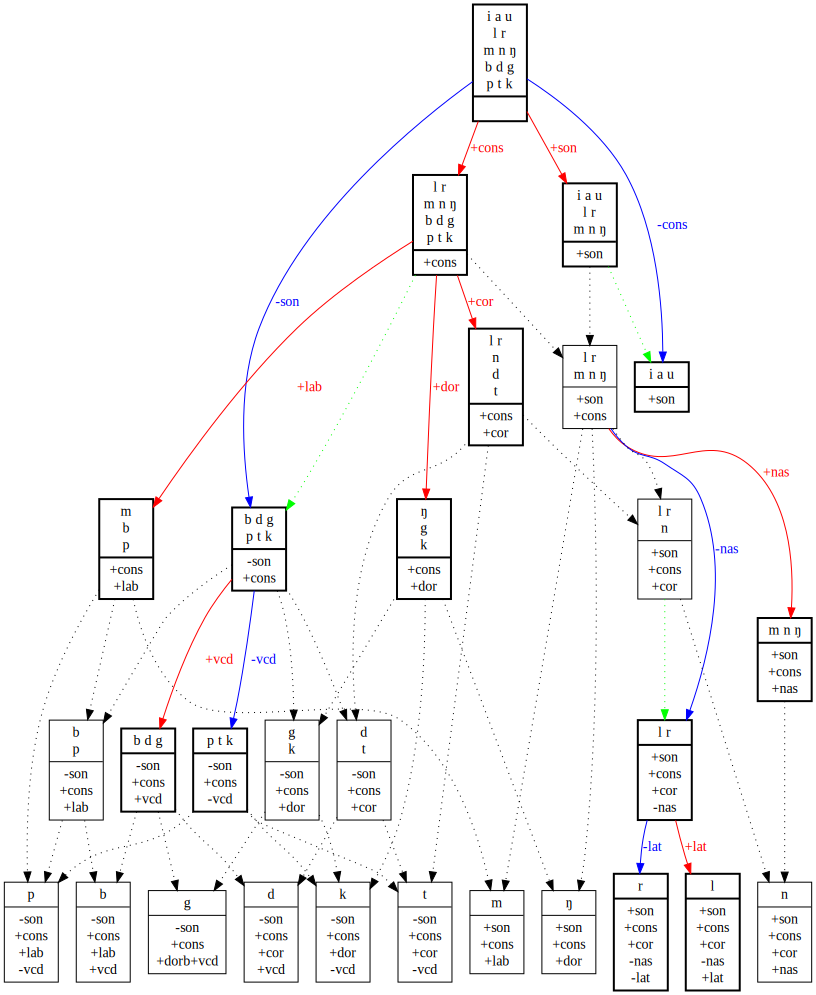
\includegraphics[width=\textwidth]{biggun.png}
  \caption{Big alphabet.}
  \label{fig:big_alphabet}
\end{figure}

The reader may be interested in investigating what happens to the `voicing' feature if the input includes the class of all phonetically voiced segments (i.e. $\Sigma \setminus \text{\{p, t, k\}}$).

It is our hope that the algorithms described in this paper might be used in generating explicitly testable empirical hypotheses on learning phonological features. Varying the input classes and the featurization method generates different predictions about the available phonological classes in a language. This is particularly true in the cases of the contrastive and full specification algorithms, where new classes are inferred based on the relationships between classes in the input. These featurizations provide a starting point for hypotheses that are testable in phonological experiments. For example, are speakers able to infer the existence of productive phonological classes for which the only evidence in the input is that the complement (with respect to some ancestor) behaves productively? 

We also note briefly that this work bears on underspecification theory \cite{Archangeli1988}. The appropriate application of underspecification has been somewhat controversial in the past \cite<e.g.>{Steriade1995}. A benefit of the algorithms presented here is that they provide a completely deterministic method for generating underspecification, depending only on the input classes and the featurization method used. This is perhaps similar to hierarchical decision-tree systems \cite<e.g.>{Dresher2003}, except that in such models, the hierarchical ordering of features must be specified by the analyst, while here it falls out naturally from the relations between the input classes. An unambiguous method for determining underspecification is doubtless of value to the field, and we leave as a question for future research how closely the methods described here line up with past analyses, and whether the predictions they make are borne out empirically.

\subsection{Feature learning}

% ROBERT: We need citations here. I think that the ``proven inadequate'' bit is a little extreme without some further justification. Were there any specific papers you had in mind?
An additional consideration associated with feature theory is that the features be learnable. There exist various proposals as to how features might be learned, e.g. from acoustic data \cite{TODO}, from articulatory data \cite{TODO}, or from distributional statistics \cite{TODO}. To date, every proposal that has been fleshed out enough to be tested has proven inadequate. It seems likely to us that progress will come from integrating multiple sources of information, with phonetic information providing a outline of possible classes, and distributional information shedding additional light on how and whether these classes (and possibly others) are used in a language. 

In any case, what must be learned under a model such as this are \textit{classes}, with features subsequently derived from their relation. Similar approaches have been proposed in the past, with classes being derived from acoustic \cite<e.g.>{Lin2005}, articulatory \cite<e.g.>{Mielke2012}, or distributional data \cite<e.g.>{GoldsmithXanthos2009, Calderone2009, Mayer2018}. Each of these approaches has been successful in certain respects, but none are completely satisfying. Methods that extract classes from phonetic data are able (in principle) to extract classes of sounds that share acoustic, articulatory, or perceptual properties, but these provide limited insights into the phonetically disparate classes described in the introduction, and into which classes are phonologically active in a particular language. Conversely, while distributional approaches have the potential (in principle) to identify both phonetically coherent and phonetically disparate classes to the extent that they are reflected in the patterning of sounds in a language, they are blind to the phonetic properties that surely inform speakers' intuitions about similarities between sounds, and suffer from the presence of distributional noise. It seems likely that the limitations of both types of models may be overcome by a model that incorporates aspects of both.

We see potential in methods like those described in a related paper by \citeA{Mayer2018}, which uses a combination of vector embedding (representing sounds numerically as points in space based on their distributional properties), Principal Component Analysis, and clustering algorithms to explicitly extract classes from a corpus. Incorporating phonetic information with distributional information may improve the performance of such models. Alternatively, a Bayesian approach, where phonetic similarity serves as an initial prior on segmental classes and considerations of their distribution inform the likelihood function, may also hold promise. A challenge for the extraction of classes from phonetic data is that classes of sounds are almost always similar only on a subset of phonetic dimensions (e.g. sonorants are articulatorily heterogeneous, but have similar acoustic properties), and the use of dimensionality reduction techniques such as Principal Component Analysis is likely to be useful in teasing apart these sources of coherence.

We see the question of how phonological classes are learned as one of great interest, and we hope that the work here serves as a useful tool in future investigations.

\FloatBarrier
\section{Conclusion}
\label{sec:conclusion}

This paper provides a detailed formalization of the properties of phonological feature systems and describes algorithms for efficiently calculating various types of featurizations of a set of input classes. An implementation of these algorithms is available for use in further research. We believe that this work provides a stronger formal grounding for the study of phonological features, and that the predictions made by the algorithms for various inputs and featurization types provide useful, testable empirical hypotheses for future experimental phonological research.

\appendix

\section{Soundness proof: Intersectional closure algorithm}
\label{app:intersectionproof}

The proof goes by induction. First, we show that every class which can be generated by the intersection of $0$ classes ($\Sigma$) or 1 class from $\mathcal C$ (i.e. $\mathcal C$ itself) belongs to $\mathcal C_\cap$. Next, we prove the induction step: if every class that can be generated by the intersection of $n$ classes from $\mathcal C$ is in $\mathcal C_\cap$, then every class that can be generated by the intersection of $n+1$ classes from $\mathcal C$ is in $\mathcal C_\cap$.

Observe that $\mathcal C_\cap$ is initialized to contain $\Sigma$. Moreover, $\mathcal Q$ is initialized to contain every class in $\mathcal C$. Each of these must be `transferred' to the intersectional closure because they do not belong to it already (dequeued from $\mathcal Q$, and appended to $\mathcal C_\cap$). This demonstrates that every intersection of 0 classes ($\Sigma$) and 1 class from $\mathcal C$ (namely, $\mathcal C$ itself) belongs to $\mathcal C_\cap$.

Now, suppose that the algorithm has guaranteed that every intersection of $n$ classes from $\mathcal C$ is in $\mathcal C_\cap$. If there exists a $Y \in \mathcal C_\cap$ which can be written as the intersection of $n+1$ classes, i.e. $Y = X_1 \cap X_2 \cap \ldots \cap X_{n+1} = Y' \cap X_{n+1}$ where $Y' = X_1 \cap X_2 \cap \ldots \cap X_n$. Since every intersection of $n$ classes is in $\mathcal C_\cap$, $Y'$ must be in $\mathcal C_\cap$. Now, regardless of whether $X_{n+1}$ was transferred from $\mathcal Q$ to $\mathcal C_\cap$ before or after $Y'$ was, there was some point at which one was in $\mathcal Q$ and the other in $\mathcal C_\cap$. When the \textbf{for} loop dequeued the one in $\mathcal Q$, it added the intersection of this one with all others in $\mathcal C_\cap$ -- i.e. $Y' \cap X_{n+1}$. Either this class was already in $\mathcal C_\cap$, or else it was not; and in the latter case, it was transferred. Thus, all sets generated by the intersection of $n+1$ classes from $\mathcal C$ are in $\mathcal C_\cap$. This completes the proof.


\section{The breadth-first algorithm for adding complement classes}
\label{app:complements}

The contrastive and full featurization algorithms add classes to $\mathcal{C_\cap}$ during their execution. In this section, we provide descriptions of the \textsc{AddComplementsContrastive} and \textsc{AddComplementsFull} algorithms introduced in Sections \ref{sec:contrastive} and \ref{sec:full}. We then motivate the use of breadth-first traversal by providing examples where traversing the classes in an arbitrary order produces spurious features, and discuss considerations on the order in which siblings are processed.

\subsection{The algorithms}

The algorithms for adding complement classes traverse $\mathcal{C_\cap}$ and, for classes with a single parent, add their complement with respect to their parent (contrastive specification) or $\Sigma$ (full specification) to the class system. In order to avoid specifying spurious features, the order in which classes are processed is crucial. Specifically, $\mathcal{C_\cap}$ must be traversed in breadth-first order: that is, processing all the siblings of a class before processing any of its children. We provide some examples where this results in more efficient feature systems in Appendix~\ref{app:bfs}. We conjecture that breadth-first traversal will always produce identical or smaller feature systems than traversal in an arbitrary order, but do not provide formal proofs here. 

In addition, siblings are processed simultaneously, and all their generated complements (if any) are added to the class system simultaneously. The motivation for this is discussed in Appendix~\ref{app:siblings}.

Below is the algorithm for \textsc{AddComplementsContrastive}:

\vspace{\baselineskip} \noindent \begin{algorithmic}
	\REQUIRE $\mathcal C_\cap$ is the intersectional closure of input class system $(\mathcal C, \Sigma)$
	\STATE
	\STATE $\mathcal Q \leftarrow \{\Sigma\}$
	\STATE
	\WHILE{$\mathcal Q \neq \varnothing$}
	\STATE $p \leftarrow \textsc{dequeue}(\mathcal Q)$
	\STATE $\textsc{Children} \leftarrow \textsc{children}(p)$
	\STATE $\textsc{ChildComplements} \leftarrow \varnothing$
	\WHILE{$\textsc{Children} \neq \varnothing$}
	\STATE $c \leftarrow \textsc{dequeue}(\textsc{Children})$
	\IF{$| \textsc{parents}(c) | = 1$}
	\STATE $\overline{c} \leftarrow p \setminus c$
	\STATE $\textsc{append}(\textsc{ChildComplements},\overline{c})$
	\ENDIF
	\ENDWHILE
	\STATE $\mathcal C_\cap \leftarrow \textsc{IntersectionalClosure}(\mathcal C_\cap, \mathcal Q' = \textsc{ChildComplements})$
	\STATE $\textsc{NewChildren} \leftarrow \textsc{children}(p)$
	\STATE $\textsc{append}(\mathcal Q, \textsc{NewChildren})$
	\ENDWHILE
\end{algorithmic}

The algorithm for \textsc{AddComplementsFull} is identical, except the complement is taken with respect to $\Sigma$ rather than the parent (i.e. the line $\overline{c} \leftarrow p \setminus c$ is replaced with $\overline{c} \leftarrow \Sigma \setminus c$).

\subsection{Breadth-first vs. arbitrary traversal}
\label{app:bfs}

Recall that a new feature only needs to be added when a class has a single parent. The contrastive and full specification algorithms add complement classes with respect to the parent and the alphabet, respectively, of classes with a single parent. These new classes alter the class structure, meaning that a class that has a single parent at one point may have two parents after a new class is added. Thus redundant classes (and hence features) may be added if a class with a single parent is processed before another class whose complement would become a parent of the first class.

Consider the input class structure in its intersectional closure shown in Figure~\ref{fig:bfs1}, and suppose we are processing it using full specification (i.e. adding complement classes with respect to $\Sigma$). 

\begin{figure}[htb!]
	\centering
	\includegraphics[width=0.2\textwidth]{bfs1.png}
	\caption{A simple class system.}
	\label{fig:bfs1}
\end{figure}

If the class \{c, e, f\} is processed before the higher class \{a, b\}, its complement with respect to $\Sigma$, \{a, b, d\} will be added to the class system. When \{a, b\} is processed later, its complement with respect to $\Sigma$, \{c, e, d, f\} is added to the class system, and becomes an additional parent to \{c, e, f\}. This results in the feature system shown in Figure~\ref{fig:bfs1feats}.

\begin{figure}[htb!]
	\centering
	\includegraphics[width=0.4\textwidth]{bfs1_feats.png}
	\caption{The classes generated after running \textsc{AddComplementsFull} if classes are processed in an arbitrary order.}
	\label{fig:bfs1feats}
\end{figure}

Note that the only purpose of F3 is to differentiate the newly added class \{a, b, d\}, whose presence is ultimately unmotivated since \{c, e, f\}, the class which generated it, ends up having two parents.

Now consider the same input, but suppose that we process \{a, b\} before \{c, e, f\} (i.e. in breadth-first order). Processing \{a, b\} adds its complement with respect to $\Sigma$, \{c, d, e, f\}, which becomes the second parent to \{c, e, f\}. Now when \{c, e, f\} is processed, its complement with respect to $\Sigma$ is not added because it does not have only a single parent. This results in the feature system shown in Figure \ref{fig:bfs2feats}.

\begin{figure}[htb!]
	\centering
	\includegraphics[width=0.4\textwidth]{bfs2_feats.png}
	\caption{The classes generated after running \textsc{AddComplementsFull} if classes are processed in breadth-first order.}
	\label{fig:bfs2feats}
\end{figure}

Note that the feature system in Figure~\ref{fig:bfs2feats} is exactly as expressive as that in Figure~\ref{fig:bfs1feats}, with the exception of the unmotivated class \{a, b, d\}. Both cover the original input. A similar example can be generated for the contrastive case.

Thus using breadth-first traversal produces a smaller featurization system that differs only in its ability to generate unmotivated classes. We conjecture that using breadth-first traversal guarantees that when a class is processed, all of its parents that will be added to the input by the end of the algorithm will have already been added, but we leave the proof as a question for future research.

\subsection{Considerations on the ordering of siblings}
\label{app:siblings}

Although breadth-first traversal gives us a rough guide for how to process classes, it does not completely determine the order. The question of the order in which siblings should be processed is still unanswered. Here, too, ordering proves to be important for the resulting class system. Consider the input shown in Figure~\ref{fig:siblinginput}, and suppose this time that we are running the contrastive specification algorithm.

\begin{figure}[htb!]
	\centering
	\includegraphics[width=0.3\textwidth]{sibling_input.png}
	\caption{A simple class system.}
	\label{fig:siblinginput}
\end{figure}

Suppose we process the class \{b\} before either of the other classes. This will result in the complement of \{b\} with respect to $\Sigma$, \{d, g\}, being added to the class system. This is shown in Figure~\ref{fig:siblingoutput1}.

\begin{figure}[htb!]
	\centering
	\includegraphics[width=0.3\textwidth]{sibling_output1.png}
	\caption{The resulting feature system when siblings are processed sequentially.}
	\label{fig:siblingoutput1}
\end{figure}

This is troubling, however, because it predicts that this class should be available in the phonology, while the similar classes \{b, g\} and \{b, d\} are not. This prediction is unmotivated by the class structure, and occurs in some form regardless of which class is processed first.

In light of this observation, and given a lack of an obvious principled way to choose which class should be processed first, we process siblings \textit{simultaneously}: that is, the complements of \textit{all} siblings are calculated, and added to the class system at the same time. In this case, the resulting class system is shown in Figure~\ref{fig:siblingoutput2}.

\begin{figure}[htb!]
	\centering
	\includegraphics[width=0.3\textwidth]{sibling_output2.png}
	\caption{The resulting feature system when siblings are processed simultaneously.}
	\label{fig:siblingoutput2}
\end{figure}

This feature system is less efficient, in the sense that it requires more features, but the overall structure is the one best motivated by the input classes. If the simpler structure in Figure~\ref{fig:siblingoutput1} is indeed the desired one, the class \{d, g\} can simply be added to the input.

When the full specification algorithm is run on the input in Figure~\ref{fig:siblinginput} with sequential processing, a similarly arbitrary class structure is generated, although in this case it involves two of the three possible two-segment subclasses rather than only one.

\bibliography{mybib.bib}
\bibliographystyle{apacite}

\end{document}
